%IMPAGINAZIONE DOCUMENTO
\documentclass[a4paper,11pt]{article}
\usepackage[margin=2.2cm]{geometry}

%% SUPPORTO A IMPAGINAZIONE
%\usepackage{lipsum}

% FONT
\usepackage[scaled]{helvet}
\usepackage[T1]{fontenc}
\renewcommand\familydefault{\sfdefault}

% CONTROLLO ORTOGRAFICO & PACCHETTI LINGUA
\usepackage[english, italian]{babel}

% FLOAT
\usepackage{float}

% TABELLE
\usepackage{tabularx}
\usepackage{booktabs}

% IMMAGINI
\usepackage{graphicx}
\graphicspath{{./diagramma/}}

% DIDASCALIE
\usepackage[labelfont={bf, small}, textfont=small]{caption}

% COLORI
\usepackage[x11names]{xcolor}

% RIFERIMENTI IPERTESTUALI
\usepackage[
	colorlinks=true,
	linkcolor=black,
	citecolor= black,
	filecolor=magenta,
	urlcolor=cyan]{hyperref}

% LISTATI
\usepackage{listings}
\usepackage{lstautogobble}
\lstset{
	backgroundcolor=\color{Snow2},
	tabsize = 4, %% set tab space width
	showstringspaces = false, %% prevent space marking in strings, string is defined as the text that is generally printed directly to the console
	numbers = left, %% display line numbers on the left
	numberstyle= \color{orange},
	commentstyle = \color{green}, %% set comment color
	keywordstyle = \color{violet}, %% set keyword color
	stringstyle = \color{SpringGreen4}, %% set string color
	rulecolor = \color{black}, %% set frame color to avoid being affected by text color
	basicstyle = \footnotesize \ttfamily , %% set listing font and size
	breaklines = true, %% enable line breaking
	numberstyle = \tiny,
	language = Java, 
	frame = bl, 
	firstnumber = 1, 
	escapeinside={(*@}{@*)},
	postbreak=\mbox{\textcolor{red}{$\hookrightarrow$}\space},
	columns=fullflexible,
	captionpos=b
}
\renewcommand{\lstlistingname}{Codice}


% METADATI RELAZIONE
\author{Diciotti Matteo}
\title{Relazione progetto AA 2023-2024 di\\ \textbf{Metodologie di Programmazione}}
\date{\today}

\begin{document}	
	\maketitle
	\vspace{1em}
	\subsubsection*{Dati autore}
	\begin{tabularx}{\textwidth}{l l >{\raggedleft\arraybackslash}X r}
		\textbf{Cognome} & \textbf{Nome} & \textbf{E-mail} & \textbf{Matricola}\\\toprule
		Diciotti & Matteo & matteo.diciotti@edu.unifi.it & 7072181
	\end{tabularx}
	\vspace{6em}
	\tableofcontents
	\vspace{1em}\noindent\rule{\textwidth}{2pt}
	
	\newpage
	\section{Presentazione progetto}
	Viene presentato nel seguito un progetto fittizio che occorre a mostrare il contesto dal quale prende spunto il codice sviluppato e in cui, ipoteticamente, si vorrebbe inserire.
	\subsection{Contesto: JDS} \label{jds}
	\textbf{J.D.S.}, ovvero \textbf{JDS is a Dispaly System}, è un software che nasce dall’esigenza di creare un ambiente di simulazione avanzato per display utilizzati in computer, console e altri dispositivi elettronici. Con l’aumento della complessità e della varietà dei display, è diventato cruciale disporre di strumenti che permettano di testare e ottimizzare le interfacce grafiche in modo efficiente e accurato. JDS si propone di fornire una piattaforma versatile e potente per la simulazione di display, consentendo agli sviluppatori di prevedere e risolvere problemi prima della fase di produzione.\\
	Le \textbf{caratteristiche principali} del software sono:
	\begin{itemize}\setlength\itemsep{-3pt}		
		\item \textbf{\underline{J}ava:} il codice è interamente scritto in linguaggio Java, fornendo ottima portabilità al sistema.
		\item \textbf{\underline{D}isplay Simulation:} Riproduzione accurata delle condizioni di visualizzazione su diversi tipi di display.
		\item \textbf{\underline{S}ystem Compatibility:} Supporto per una vasta gamma di dispositivi, dai computer ai dispositivi mobili.
		\item \textbf{In-depth Analysis:} Funzionalità di monitoraggio e reportistica per identificare e risolvere problemi di performance e qualità.
		\item \textbf{Scalability:} Capacità di adattarsi a progetti di qualsiasi dimensione e complessità.
	\end{itemize}	
	\subsection{Inserimento del progetto in JDS} \label{jds:inserimento-elaborato}
	Il progetto presentato al punto precedente si compone di varie parti che cooperano tra loro. In questo contesto possiamo identificare il posizionamento dell'elaborato come la parte centrale del sistema, la parte che implementa i concetti di display e parte dei servizi propri dei sistemi operativi interni agli stessi display. Non vengono quindi prese in considerazione, nel progetto sviluppato, le caratteristiche di reportistica e monitoraggio o strumenti di simulazione avanzati.
		
	\section{Specifiche Java}
	L'elaborato è stato implementato e testato attraverso l'utilizzo dell'IDE Eclipse, versione Linux 2024-06 (4.32.0) (fino alla versione Java \texttt{java.verision=21.0.4}), sul sistema Kubuntu, kernel \texttt{6.8.0-38-generic} e utilizzando per il progetto la versione 11 di Java (\texttt{java-11-openjdk-amd64}).
	Per i test sono stati utilizzati i framework JUnit4 e AssertJ\footnote{Il framework AssertJ non è presente tra le librerie standard di Java, quindi è stato inserito come libreria aggiuntiva all'indirizzo ''\texttt{\$ROOT\_PROJECT\_DIRECTORY/test-libs/assertj-core-3.26.0.jar}'' e inserita nel buildpath del progetto Eclipse.}.
	
	\section{Funzionalità del progetto}
	Il progetto implementa, come detto, un sistema per la simulazione della gestione di display.\\
	I display possono avere nessuno, uno o più sensori, come per esempio un sensore di luminosità esterna, al fine di impostare automaticamente la luminosità dello schermo, o un orologio, al fine di modificare la gamma di colori durante le ore notturne.\\
	Ogni display può incorrere in malfunzionamenti, è quindi stato implementato un meccanismo di controllo dei malfunzionamenti, in particolare per intercettare un cambio inatteso della risoluzione dello schermo o una disconnessione improvvisa di un'interfaccia video.\\
	Infine, ogni display dovrà proiettare, attraverso un cavo/canale sullo schermo un flusso di frame ricevuti da un'interfaccia video o dei comandi predefiniti. Questi frame possono essere semplici o composti, ovvero possono rappresentare un tipico schermo di un dispositivo, oppure possono essere composti in vari modi, generando quindi un mosaico di frame.
	
	\section{Diagramma UML}
	Si mostra a pagina \pageref{fig:classdiagram} il diagramma UML delle classi\footnote{Per una migliore visione dei diagrammi presenti nella relazione si consulti l'allegato \href{../AllDiagrams.pdf}{AllDiagrams.pdf}.}.\\
	\begin{figure}[p]
		\noindent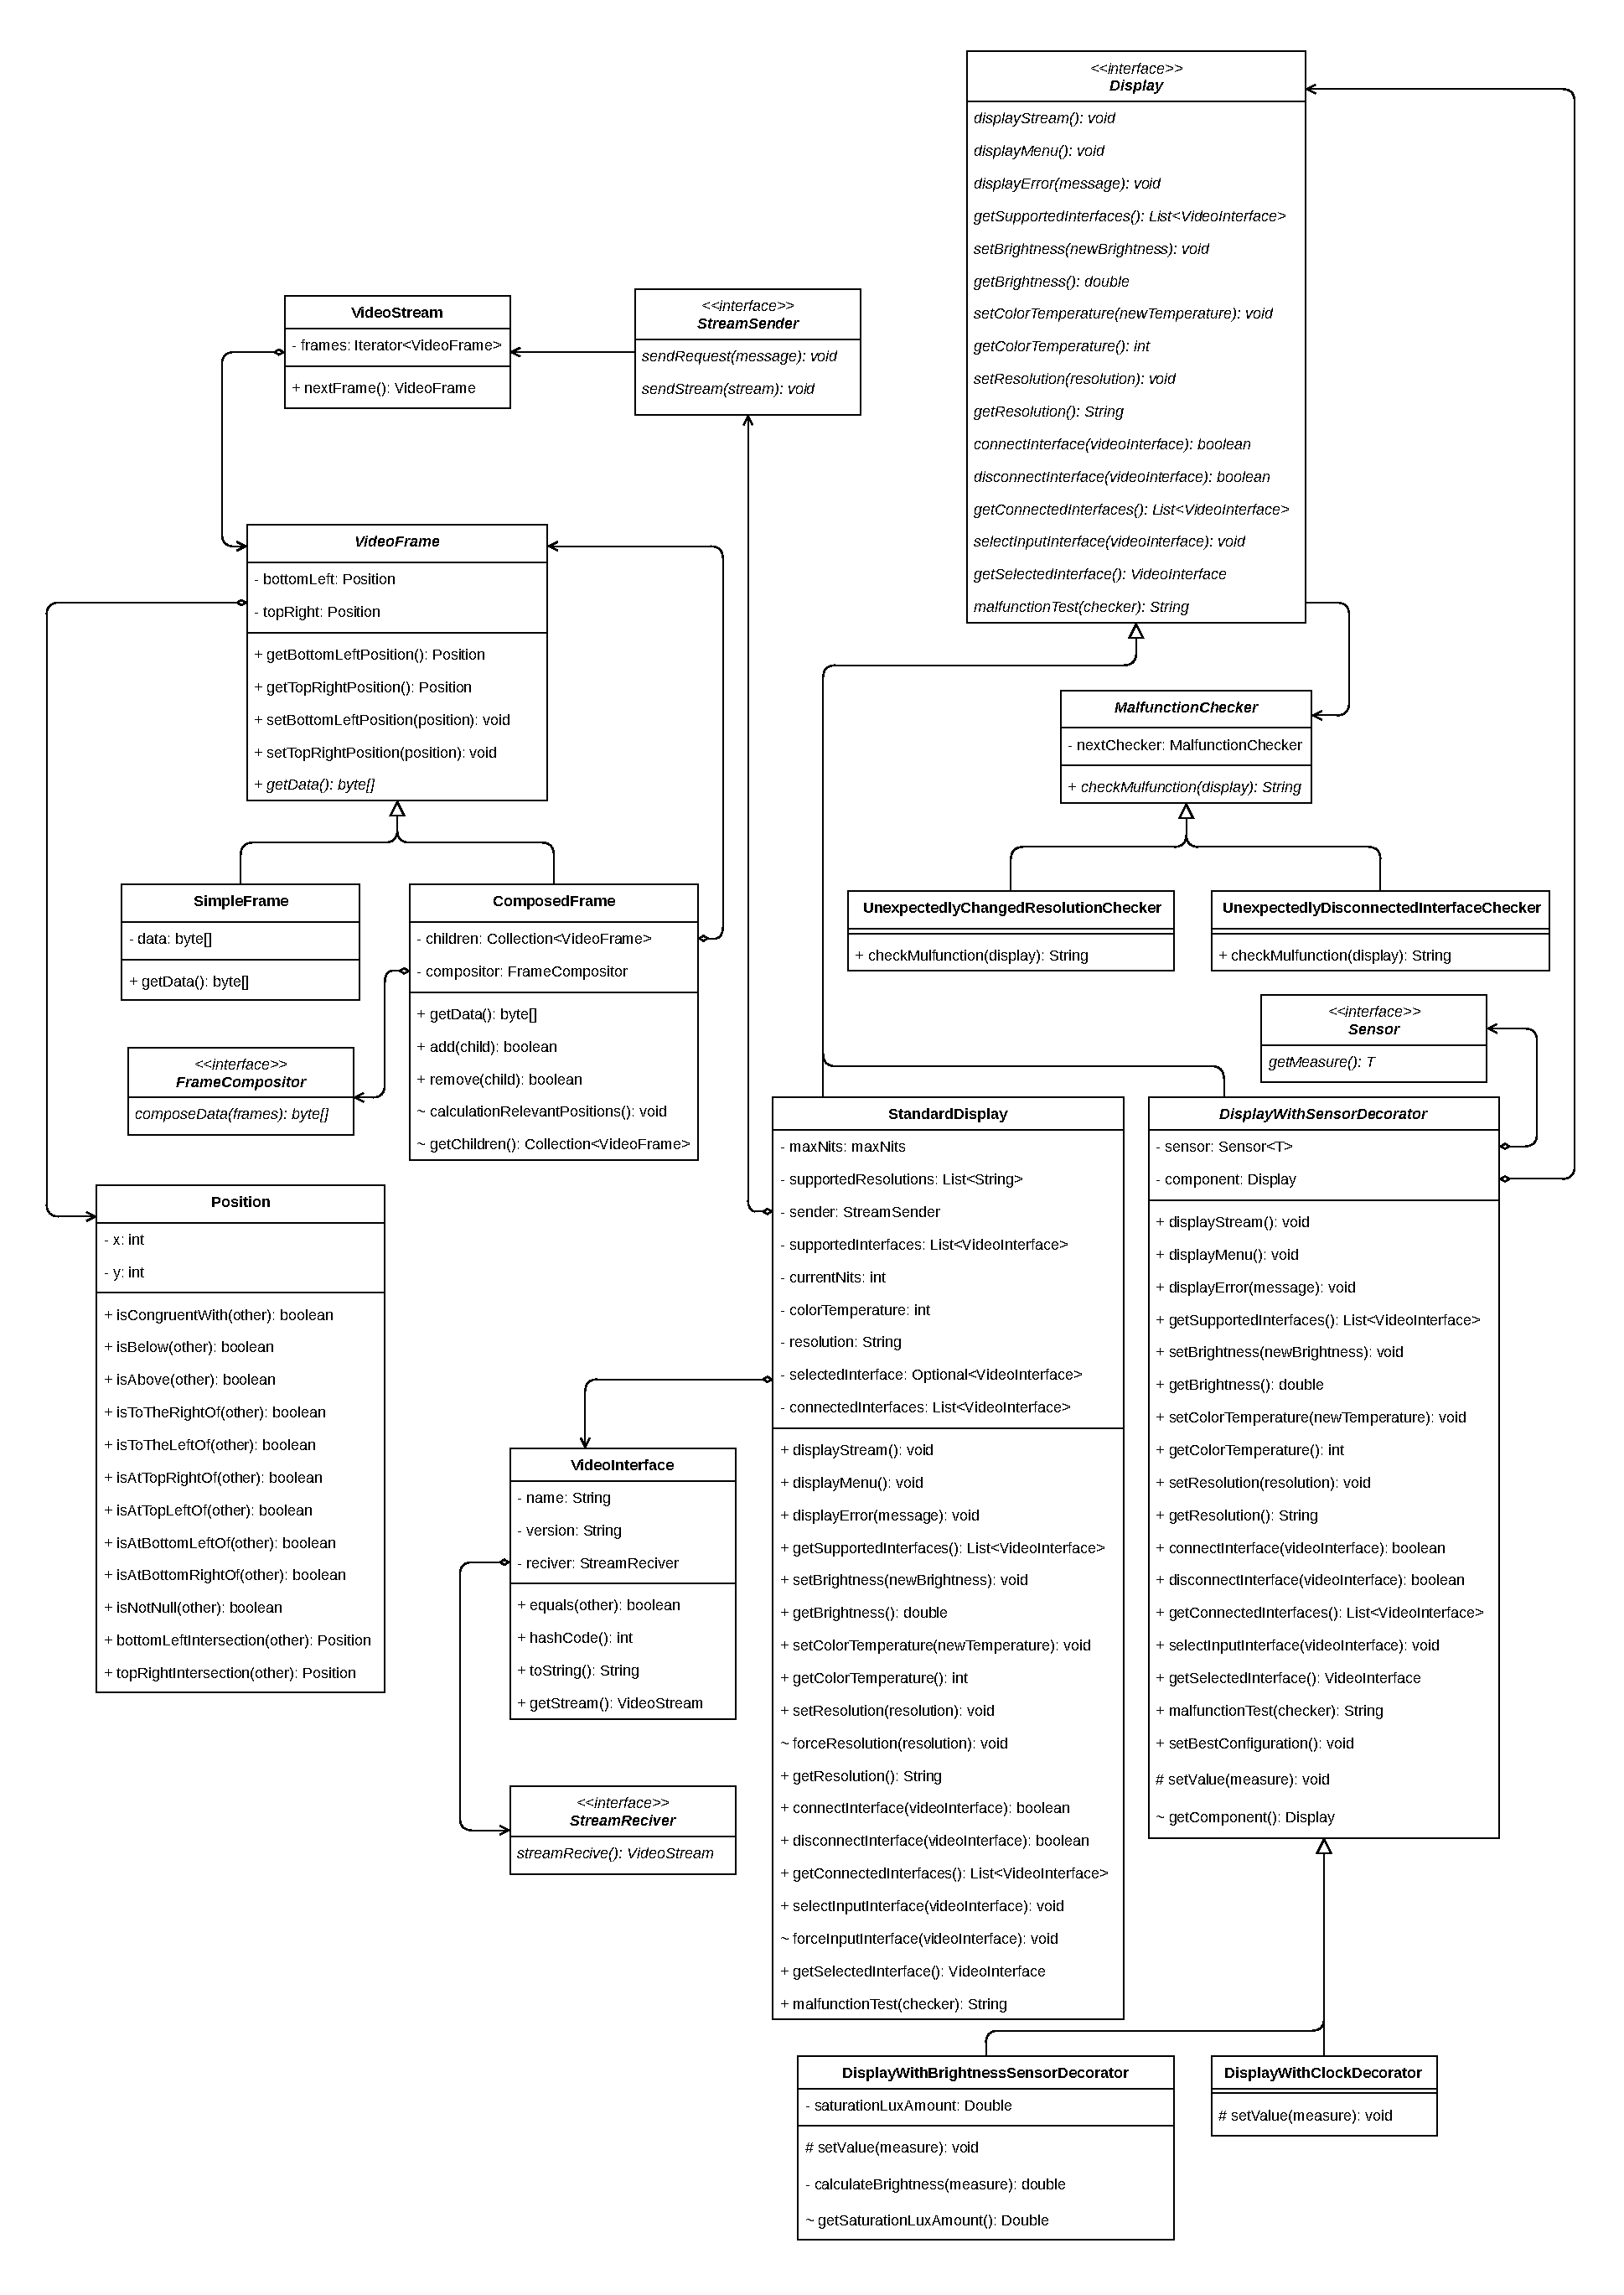
\includegraphics[width=\textwidth]{diagramma/ClassDiagramm-Types.pdf}
		\captionof{figure}{Diagramma delle classi descritto con \textit{Unified Modelling Language}.}
		\label{fig:classdiagram}
	\end{figure}
	
	\section{Lista pattern implementati}
	\begin{itemize}
		\item Decorator, versione con un'unica responsabilità;
		\item Template Method;
		\item Chain of Responsability;
		\item Composite, variante type safe.
	\end{itemize}
	
	\section{Descrizione scelte di design}
	\subsection{Gerarchia \texttt{Display}, \texttt{Sensor} e \texttt{StreamSender}}
	Per l'implementazione di \texttt{Display} è stato utilizzato il pattern \textbf{Decorator}\footnote{Tutta la nomenclatura per la descrizione dei componenti dei pattern proviene dal manuale \textit{Design patterns: elements of reusable object-oriented software}, {\fontfamily{bch}\selectfont G.O.F.}.} per l'aggiunta di un'unica responsabilità, ovvero la gestione di sensori. Il motivo primario che ha portato alla decisione di utilizzare il pattern è la grande varietà di sensori che possono essere associati ad un display, permettendo la creazione dinamica di innumerevoli display in base alle combinazioni di sensori.\\
	L'oggetto da decorare, il \textit{ConcreteComponent}, risulta essere \texttt{StandardDisplay} mentre l'unico \textit{Decorator} risulta essere \texttt{DisplayWithSensorDecorator}.\\
	I metodi decorati sono \textit{displayStream()}, \textit{displayMenu()} e \textit{displayError(message)} ai quali viene aggiunta la richiesta di impostare preventivamente la miglior configurazione degli attributi del display in base ai valori ottenuti dal sensore presente (vedi metodo \textit{setBestConfiguration()}).\\
	Il motivo per cui \texttt{DisplayWithSensorDecorator} è un'astrazione e le sottoclassi non sono state implementate come \textit{ConcreteDecorator} nasce dalla volontà di ridurre la duplicazione di codice, implementando direttamente le operazioni ereditate da \texttt{Display} nella classe base e astraendo solo le operazioni strettamente dipendenti dai sensori, ovvero astraendo \textit{setValue()}, implementando quindi il metodo nelle classi concrete \texttt{DisplayWithClockDecorator} e \texttt{DisplayWithBrightnessSensorDecorator}. Così facendo viene riutilizzato il codice del decoratore per ogni tipologia di sensore. Attraverso l'uso del pattern \textbf{Template Method} è stato possibile definire un algoritmo comune per il metodo \textit{setBestConfiguration()}, il template method (definito \textcolor{violet}{\texttt{final}} nella classe astratta), che richiamasse la funzione \textit{setValue()}, implementata dalle sottoclassi (unico metodo da implementare per creare una classe di tipo \texttt{DisplayWithSensorDecorator} e quindi per aggiungere un nuovo tipo di sensore al dispositivo).\\
	Inoltre le classi presenti nel sistema che implementano \texttt{DisplayWithSensorDecorator} utilizzano nel metodo \textit{setValue()} dei valori predefiniti per il calcolo. Questa caratteristica è modificabile e deriva dal contesto, si può prevedere una comoda modifica che permetta la specificazione delle variabili in modo che il calcolo sia caratteristico per ogni sensore e per ogni display.\\
	Infine, a proposito di \texttt{DisplayWithBrightnessSensorDecorator} e del metodo \textit{setValue()}, è stato implementato un semplice algoritmo di calcolo lineare, ma attraverso l'utilizzo del pattern \textbf{Strategy} (\underline{non} implementato) potevano essere create varie tipologie di algoritmo (lineare, logaritmico, ecc..) in modo che fosse possibile differenziare ulteriormente i display e i loro meccanismi di funzionamento.
	Tale aggiunta può quindi essere presa in considerazione per raffinazioni future dell'algoritmo di impostazione automatica della luminosità.\\
	Non avendo implementato un meccanismo di logging, il metodo \textit{DisplayWithSensorDecorator.setBest-Configuration()} (così come i metodi \textit{MalfunctionChecker.checkMalfunction($\cdot$)} che vedremo in seguito) al momento stampa le eccezioni pervenute dai sensori sulla console. Si prevede una modifica del codice nel senso della creazione di un report complessivo del sistema, ma che risultava non utile al fine dell'elaborato.\\
	Infine, sempre dettata dal contesto in cui si inserisce l'elaborato, è stata utilizzata una semplificazione per la proiezione dei frame sul display, ovvero vengono passati flussi o comandi all'interfaccia \texttt{StreamSender}, la quale poi avrà il compito di gestire le richieste\footnote{Nei seguenti diagrammi sono stati inseriti solo una parte dei campi, solo quelli che sono stati ritenuti essere fondamentali per la comprensione delle gerarchie.}.\\
	\begin{minipage}[c]{\textwidth}
		\centering
		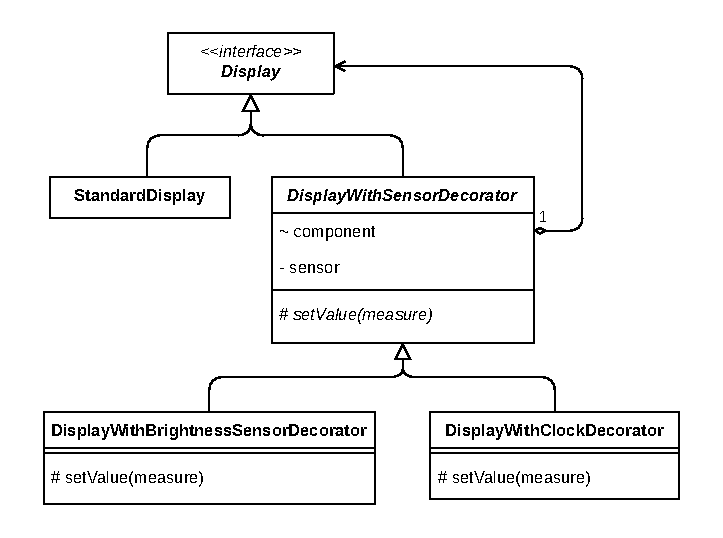
\includegraphics[width=.5\textwidth]{diagramma/ClassDiagramm-DisplayHierarchy.pdf}
		\captionof{figure}{Gerarchia \texttt{jds.display.Display}.}
		\label{fig:display}
	\end{minipage}	
	
	\subsection{Gerarchia \texttt{MalfunctionChecker}}
	Per il controllo dei malfunzionamenti dei display è stato implementato il pattern \textbf{Chain of Responsibility}, al fine di poter aggiungere controlli dinamicamente e di poter personalizzare la catena in base allo specifico display. Il pattern ha come \textit{Handler} la classe \texttt{MalfunctionChecker} e le sottoclassi rappresentano i \textit{ConcreteHandler} che implementano gli specifici controlli da effettuare.\\
	L'accertamento viene affidato da un oggetto \texttt{Display} a un oggetto di tipo \texttt{MalfunctionChecker} che non se ne occupa direttamente ma che trasmette la richiesta alle sottoclassi. Solo in caso di mancata gestione da parte di una sottoclasse viene chiamato in causa il codice della classe base la quale passa la richiesta al successivo membro della catena oppure restituisce una stringa per specificare l'assenza di malfunzionamenti noti.\\
	\begin{minipage}[c]{\textwidth}
		\centering
		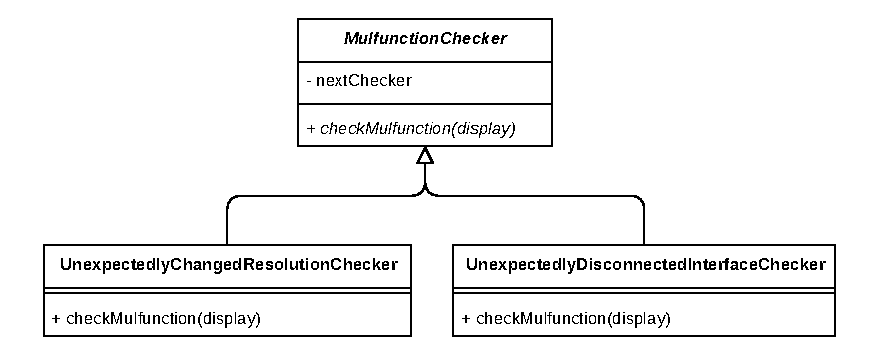
\includegraphics[width=.5\textwidth]{diagramma/ClassDiagramm-MalfunctionChecker.pdf}
		\captionof{figure}{Gerarchia \texttt{jds.display.Malfunction.MalfunctionChecker}.}
		\label{fig:malfunction}
	\end{minipage}
	
	\subsection{\texttt{VideoInterface}}
	Nel progetto non è stata considerata la componente audio e così facendo è stato ritenuto non essere necessario implementare le interfacce video come oggetti staticamente differenti nel sistema, data la scarsa distinzione a livello di operazioni tra le classi nel sistema, ma queste sono state distinte attraverso degli attributi nella classe \texttt{VideoInterface}, nella quale è stato sovrascritto il metodo \textit{equals($\cdot$)} per controllare l'uguaglianza tra due oggetti. Si può comunque prevedere una ristrutturazione del codice nel senso della definizione e specifica delle interfacce video e audio con annesse le varie caratteristiche che possiedono.\\
	\lstinputlisting[firstline=8, lastline=25, caption={Attributi e costruttore della classe \texttt{jds.display.interfaces.VideoInterface}.}, label=lst:videointerface]{../src/jds/display/interfaces/VideoInterface.java}

	
	\subsection{\texttt{VideoStream} e gerarchia \texttt{VideoFrame}}
	Infine, è stato utilizzato il pattern \textbf{Composite} per rappresentare la struttura dei frame di uno stream video. La classe \textit{StreamVideo} possiede un riferimento ad un iteratore di \texttt{VideoFrame} i quali possono restituire le informazioni sui pixel in forma di vettore di byte. I \texttt{VideoFrame} sono staticamente suddivisi tra \texttt{SimpleFrame} e \texttt{ComposedFrame}, dove i primi contengono un vettore di byte il quale rappresenta il contenuto dei pixel del frame, mentre i frame composti sono la composizione su due dimensioni dei frame semplici (e di altri frame composti). La classe \texttt{SimpleFrame} rappresenta l'unica classe \textit{Leaf} del pattern Composite, mentre la classe \texttt{ComposedFrame} rappresenta la classe \textit{Composite}. Il supertipo comune, ovvero il \textit{Component} del pattern, è l'interfaccia \texttt{VideoFrame}. 
	Come prevede il pattern, prima che i \texttt{ComposedFrame} rimandino la richiesta per l'ottenimento delle informazioni sui pixel ad un'interfaccia \texttt{FrameComposer}, che ha il compito di creare attraverso qualche specifico algoritmo un array di byte che rappresenti le informazioni sui pixel della composizione, richiedono ai figli, attraverso la medesima operazione \textit{getData()}, i dati necessari alla composizione.\\
	Infine, va osservato che la variante implementata è quella incline alla sicurezza dei metodi, cioè quella che evita errori al momento dell'esecuzione. Per questo motivo la presenza dei metodi \textit{add(child)}, \textit{remove(child)} eccetera è esclusiva della classe concreta \texttt{ComposedFrame}.\\
	\begin{minipage}[c]{\textwidth}
		\centering
		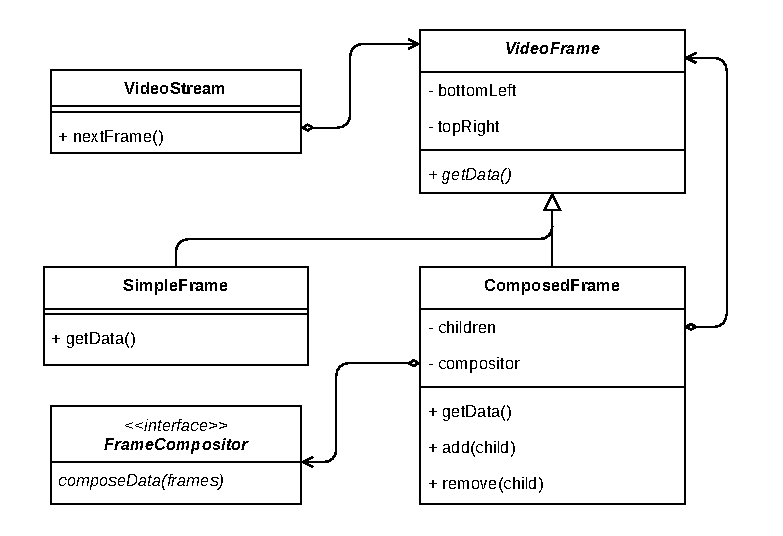
\includegraphics[width=.5\textwidth]{diagramma/ClassDiagramm-VideoStream.pdf}
		\captionof{figure}{\texttt{jds.display.videostream.VideoStream} e gerarchia \texttt{jds.display.videostream.VideoFrame}.}
		\label{fig:videostream}
	\end{minipage}
	
	\section{Test}
	Si presentano nel seguito una serie di note preliminari che sono generali per tutto l'elaborato:
	\begin{itemize}\setlength\itemsep{-3pt}
		\item I test sono stati scritti in forma non completamente estesa, ovvero inserendo più asserzioni all'interno di un unico JUnitTest per controllare la correttezza di un intero metodo del \textit{Software Under Test} (o \textit{SUT}) e non il singolo comportamento di questo. È stato ritenuto che la metodologia fosse accettabile dato il contesto, in quanto vengono comunque testati separatamente i metodi del SUT, permettendo l'identificazione dell'origine dei fallimenti, ma vengono tenuti uniti i test dei vari comportamenti del singolo metodo, limitando l'eccessiva produzione di micro-JUnitTest.
		\item È stato deciso di non utilizzare \texttt{extracting(String)} e \texttt{hasFieldOrPropriety(String)} (e affini), metodi di \texttt{assertj}, per testare lo stato di oggetti poiché questi, sebbene siano metodi molto potenti, hanno il difetto di rompersi dopo che dei campi testati vengono rinominati, facendo venir meno uno dei principi dei test e del refactoring\footnote{Il metodo \texttt{org.assertj.core.api.Assertions.assertThat(.)} è deprecato solo per alcuni tipi dei parametri (si può notare dall'IDE che lo segnala contestualmente al comando di \textcolor{violet}{\texttt{import}}). I metodi utilizzati nel progetto possiedono un nome equivalente a quello presentato ma una firma differente: questi non risultano deprecati (si può infatti notare che l'IDE non li barra direttamente nel codice). Si veda a proposito la \href{https://www.javadoc.io/doc/org.assertj/assertj-core/3.26.0/org/assertj/core/api/Assertions.html}{documentazione della libreria \texttt{assertJ}}.}.
		\item È stato ritenuto che testare i metodi auto-generati dall'IDE, ovvero getters e setters ai quali non è stata aggiunta ulteriore logica, non fosse determinante e che aumentava inutilmente la dimensione dell'elaborato. Questa decisione è stata presa con la consapevolezza che, in un contesto non accademico, sarebbe stato preferibile implementarli comunque per verificare la correttezza dei metodi in futuro, nel caso in cui venisse aggiunta logica non testata.
		\item Il motivo per cui sono presenti dei metodi definiti package-private (visibili a fig. \ref{fig:classdiagram} con simbolo \textbf{\textasciitilde}) è da far risalire all'utilizzo di questi all'interno dei test: nessun metodo definito package-private è stato utilizzato direttamente all'interno delle classi del medesimo pacchetto, è stata sempre utilizzata l'interfaccia pubblica (public e protected) delle classi. 
	\end{itemize}
	
	Per testare il progetto sono state implementate all'interno della cartella sorgente \textit{tests} le classi fittizie \texttt{jds.MockStreamReciver}, \texttt{jds.MockStreamSender} e \texttt{jds.videostream.MockFrameCompositor}, servizi non implementati del sistema, e la classe \texttt{DisplaySetterToTestMalfunctions} che occorre nelle classi di test della gerarchia \texttt{MalfunctionChecker} per settare direttamente alcuni campi di display al di fuori dal pacchetto in cui risiede la classe \texttt{StandardDisplay}.
	
	\subsection{Gerarchia \texttt{Display}}
	Per testare la gerarchia Display è necessario testare i pattern \textbf{Decorator} e \textbf{Template Method}.
	Si è testato innanzitutto la classe \texttt{StandardDisplay}, ovvero il componente da decorare, attraverso test che per ogni metodo ne valutassero il corretto funzionamento, sia per il lancio di eccezioni (attraverso il metodo \textit{assertThatThrownBy($\cdot$)} e l'utilizzo di lambda) che per il corretto svolgimento delle operazioni attese.\\
	In secondo luogo si è passati a testare la classe \texttt{DisplayWithSensorDecorator} attraverso le classi di test delle sottoclassi che la implementano, ovvero \texttt{DisplayWithBrightnessSensorDecoratorTest} e \texttt{DisplayWithClockDecoratorTest}.
	Per creare delle implementazioni di \texttt{Sensor}, invece di produrre classi aggiuntive, dato che \texttt{Sensor<T>} è un'interfaccia funzionale, sono state assegnate delle lambda expressions con cast a sensori.\\
	In queste classi e stato testato su una catena di 2 decoratori (differenti) e un componente che il comportamento dei metodi decorati ovvero \textit{displayStream()}, \textit{displayMenu()} e \textit{displayError(message)}, modificasse lo stato dell'oggetto \textit{component} alla base della "catena" di decoratori e che poi passasse la richiesta al successivo \textit{decorator} o al \textit{component}. Per tutti gli altri metodi è stato testato che venisse passata la richiesta al \textit{component} senza svolgere ulteriori operazioni (e che quindi le eccezioni lanciate fossero uguali o che il risultato di un metodo fosse uguale al risultato del metodo chiamato sul \textit{component}).
	Sono state inoltre testate le due implementazioni del metodo \textit{setValue()} per accertare la correttezza del pattrern template method, oltre ovviamente al metodo \textit{setBestConfiguration()}.
	
	\subsection{Gerarchia \texttt{MalfunctionChecker}}
	Per testare che il pattern \textbf{Chain of Responsability} abbia il corretto funzionamento si controlla nelle classi di test \texttt{UnexpectedlyChangedResolutionCheckerTest} e {\texttt{UnexpectedlyDisconnectedInterface}- \texttt{CheckerTest}} che, se la classe deve gestire la richiesta e attualmente non può/sa farlo allora la passi al successivo \textit{ConcreteHandler}, altrimenti si controlla che restituisca il valore atteso.
	\lstinputlisting[firstline=45, lastline=60, caption={Test per la classe \texttt{jds.display.malfunction.UnexpectedlyChangedResolutionCheckerTest}.}, label=lst:test-changed-resolution]{../tests/jds/display/malfunction/UnexpectedlyChangedResolutionCheckerTest.java}
	
	\subsection{\texttt{VideoInterface}}
	Nella classe \texttt{VideoInterface} è stato testato il corretto funzionamento dei metodi utilizzando le medesime tecniche utilizzate per le classi precedenti. In particolare sono stati testati i metodi \textit{equals($\cdot$)}, \textit{hashCode()} e \textit{toString()} secondo quanto atteso in letteratura (\textit{equals} risultante \textcolor{violet}{false} in caso di \texttt{other} assegnato a \textcolor{violet}{null}, \textit{hashCode} uguale per elementi uguali, eccetera).
	\lstinputlisting[firstline=43, lastline=60, caption={Test del metodo \textit{equals(other)} per la classe \texttt{jds.display.interfaces.VideoInterface}.}, label=lst:test-videointerface-equals]{../tests/jds/display/interfaces/VideoInterfaceTest.java}
	
	\subsection{\texttt{VideoStream} e gerarchia \texttt{VideoFrame}}
	Una volta testata la classe \texttt{Position} con tecniche non dissimili da quelle precedentemente utilizzate, testando per ogni metodo che il risultato atteso sia coerente con quello ottenuto, si eseguono i test per \texttt{SimpleFrame}, ovvero si testa quel minimo di logica dei setters.\\
	Si è testata successivamente la classe \texttt{ComposedFrame}, utilizzando la classe \texttt{MockFrameCompositor}. Dato che si tratta di un pattern \textbf{Composite} si testa che il metodo \textit{getData()}, operazione astratta della classe base, sia passata dal \textit{Composite} ai figli, e che quindi, in questo caso per come è stata implementata la classe \texttt{MockFrameCompositor}, che il risultato ottenuto contenga tutte le istanze dei dati dei figli.
	\lstinputlisting[firstline=66, lastline=75, caption={Test del metodo \textit{getData()} per la classe \texttt{jds.display.videostream.ComposedFrame}.}, label=lst:test-composedframe-getdata]{../tests/jds/videostream/ComposedFrameTest.java}
	
	Infine è stata testata la classe \texttt{VideoStream} affinché fosse confermato che il metodo \textit{nextFrame()} restituisse sempre il corretto frame.
	\lstinputlisting[firstline=53, lastline=64, caption={Test del metodo \textit{nextFrame()} per la classe \texttt{jds.display.videostream.VideoStream}.}, label=lst:test-videostream-nextframe]{../tests/jds/videostream/VideoStreamTest.java}
	
\end{document}

